% !TEX TS-program = pdflatex
% !TEX encoding = UTF-8 Unicode

% This file is a template using the "beamer" package to create slides for a talk or presentation
% - Giving a talk on some subject.
% - The talk is between 15min and 45min long.
% - Style is ornate.

% MODIFIED by Jonathan Kew, 2008-07-06
% The header comments and encoding in this file were modified for inclusion with TeXworks.
% The content is otherwise unchanged from the original distributed with the beamer package.

\documentclass{beamer}


% Copyright 2004 by Till Tantau <tantau@users.sourceforge.net>.
%
% In principle, this file can be redistributed and/or modified under
% the terms of the GNU Public License, version 2.
%
% However, this file is supposed to be a template to be modified
% for your own needs. For this reason, if you use this file as a
% template and not specifically distribute it as part of a another
% package/program, I grant the extra permission to freely copy and
% modify this file as you see fit and even to delete this copyright
% notice. 


\mode<presentation>
{
  \usetheme{Pittsburgh}
  % or ...

  \setbeamercovered{transparent}
  % or whatever (possibly just delete it)
}


\usepackage{fontspec}
\setmainfont{Times New Roman}

\usepackage{graphicx}
\usepackage{wrapfig}

\usepackage[portuguese]{babel}
% or whatever

\usepackage{pgf}
\usepackage{tikz}
\usetikzlibrary{arrows,automata}

\usepackage[utf8]{inputenc}
% or whatever

%\usepackage{times}

% Or whatever. Note that the encoding and the font should match. If T1
% does not look nice, try deleting the line with the fontenc.


\title[Short Paper Title] % (optional, use only with long paper titles)
{Utilização de técnicas de Machine Learning e PLN para a criação de um Bot}

%\subtitle
%{Presentation Subtitle} % (optional)

\author[Carlos] % (optional, use only with lots of authors)
{Carlos António Senra Pereira\inst{1} } %\and S.~Another\inst{2}}
% - Use the \inst{?} command only if the authors have different
%   affiliation.

\institute[Universidade do Minho] % (optional, but mostly needed)
{
  \inst{1}%
  Mestrado em Matemática e Computação\\
  Departamento de Matemática\\
  Universidade do Minho
}
  %\and
  %\inst{2}%
  %Department of Theoretical Philosophy\\
  %University of Elsewhere}
% - Use the \inst command only if there are several affiliations.
% - Keep it simple, no one is interested in your street address.

\date[Short Occasion] % (optional)
{\today}

\subject{Talks}
% This is only inserted into the PDF information catalog. Can be left
% out. 



% If you have a file called "university-logo-filename.xxx", where xxx
% is a graphic format that can be processed by latex or pdflatex,
% resp., then you can add a logo as follows:

% \pgfdeclareimage[height=0.5cm]{university-logo}{university-logo-filename}
% \logo{\pgfuseimage{university-logo}}



% Delete this, if you do not want the table of contents to pop up at
% the beginning of each subsection:
\AtBeginSubsection[]
{
  \begin{frame}<beamer>{Conteúdos}
    \tableofcontents[currentsection,currentsubsection]
  \end{frame}
}


% If you wish to uncover everything in a step-wise fashion, uncomment
% the following command: 

%\beamerdefaultoverlayspecification{<+->}


\begin{document}

\begin{frame}
  \titlepage
\end{frame}

\begin{frame}{Conteúdos}
  \tableofcontents
\end{frame}


\section{Introdução}
\begin{frame}{Introdução}
\hspace{11pt} O processamento de Linguagens Naturais é bastante complexo, e ainda mais no ponto de vista de uma máquina determinística.\\
\vspace{2mm}
Por isso, utilizando técnicas de Machine Learning é possível construir modelos capazes de analisar e frases e tomar ações com bastante precisão. \\
\vspace{2mm}
\hspace{11pt}Utilizando Padrões Linguísticos e sistemas de reescrita, podemos criar assim um Bot onde a análise é feita num domínio de pesquisa ou aplicação definido pelo utilizador, através dos Padrões Linguísticos definidos no Modelo do Bot.

\end{frame}

\subsection{Estrutura}
\begin{frame}{Introdução - Estrutura do Bot}

\begin{center}
\begin{tikzpicture}[->,>=stealth',shorten >=1pt,auto,node distance=2.8cm,
                    semithick]
  \tikzstyle{every state}=[fill=white,sloped]

  \node[state]          (D)                   {RS};
  \node[initial,state] (A) [below left of=D]  {Input};
  \node[state]         (C) [below right of=D] {Output};

  \path 
        (A) edge                    node {parsing(s)} (D)
        (D) edge                    node {reação(ões)} (C)
             edge [loop above] node {} (B);
\end{tikzpicture}
\end{center}

\begin{itemize}
\item RS: Representações Semânticas
\end{itemize}

\end{frame}

%%%%%%%%%%%%%%%%%%%%%%%%%%%%%%%%%%%%%%%%%%%%%%%%%%%%%%%%%
%%%%%%%%%%%%%%%%%%%%%%%%%%%%%%%%%%%%%%%%%%%%%%%%%%%%%%%%%

\subsection{Objetivos}

\begin{frame}{Objetivos}

%Rever os objetivos para dar um sentido e uma ideia mais direta do que se está a fazer.

%\begin{enumerate}
%\item Construir uma aplicação capaz de analisar e reconhecer frases introduzidas por utilizadores; \pause
%\item Através de um modelo de Machine Learning, analisar essas frases; \pause
%\item Utilizando técnicas de Machine Learning em conjunto com bases de dados de conhecimento, criar um modelo capaz de classificar uma análise e atribuir uma ação. \pause
%\item Construir relações entre sujeito e objeto e através dessas mesmas, gerar todas(ou quase todas) as expressões regulares correspondentes. \pause
%\end{enumerate}

\begin{enumerate}
\item Desenvolver uma aplicação de Chat; \pause
\item Utilizar o FreeLing para analisar frases e devolver o PoS e as dependências sintáticas; \pause
\item Criar um modelo linguístico para permitir o uso de padrões linguísticos e sistemas de reescrita; \pause
%Assim o Bot fica com capacidade de interpretar e reconhecer padrões e adaptar-se
\item Construir uma base de dados capaz de armazenar conhecimento para a aprendizagem; \pause
\item Escrever uma função para extrair e/ou combinar $features$ da análise de uma frase; \pause
\item Definir um modelo de Machine Learning para classificar a ação a tomar após a análise; \pause
\item Definir ontologias para gerar expressões relativas a um certo domínio de pesquisa ou aplicação.
\end{enumerate}

\end{frame}

%%%%%%%%%%%%%%%%%%%%%%%%%%%%%%%%%%%%%%%%%%%%%%%%%%%%%%%%%
%%%%%%%%%%%%%%%%%%%%%%%%%%%%%%%%%%%%%%%%%%%%%%%%%%%%%%%%%

\section{Descrição abstrata do modelo}

\subsection{Modelo}
\begin{frame}{Modelo}
\hspace{11pt} Após a análise do problema em questão, foi criado um modelo de um Bot.\\

\begin{align*}
Bot &::= Regra^* 
\end{align*}
\begin{align*}
Regra ::= ( \quad antecedente & : ERL \quad , \\
\text{ reação} & : FR^* \quad  )
\end{align*}

Onde:
\begin{enumerate}
\item $FR$: Função de Reação; \\
\item $ERL$: Expressão Regular Linguística. \\
\end{enumerate}

%\hspace{11pt} Com este modelo, é possível escrever uma álgebra de Bot's que permite o uso dos mesmos numa solução, por exemplo, em paralelo, em sequência, etc.

\end{frame}

%%%%%%%%%%%%%%%%%%%%%%%%%%%%%%%%%%%%%%%%%%%%%%%%%%%%%%%%%
%%%%%%%%%%%%%%%%%%%%%%%%%%%%%%%%%%%%%%%%%%%%%%%%%%%%%%%%%

\subsection{Expressões Regulares Linguísticas}

\begin{frame}{Expressões Regulares Linguísticas}{Exemplo}
Comecemos com um exemplo prático do nosso modelo:

\begin{align*}
&pergunta\_pessoa = \{exp: [ &&\\
&\qquad (\backslash w^*, \quad pronome\_geral, && None),\\
&\qquad (\backslash w^*, \quad verbo\_geral, && None),\\
&\qquad (\backslash w^*, \quad nome\_proprio\_geral, && name),\\
&\qquad (.^*, \quad pergunta, && None)\\
&], action: [pergunta\_pessoa] \} &&
\end{align*}

\end{frame}

\begin{frame}{Expressões Regulares Linguísticas}{Abstração}

\hspace{11pt} Estas são as expressões definidas serão compiladas e interpretadas pelo Bot. \\

\begin{align*}
ERL &  ::=  EL^*   \\
EL & ::= ( IT^*, \quad FR^* )\\
IT  &::= ( pal : ER, \quad tag : ER, \quad catch : palavra ) \\
FR &::= \text{Função}
\end{align*}

Onde:
\begin{enumerate}
\item $ER$: Expressão Regular;\\
\item $pal$: palavra; \\
\item $tag$: PoS; \\
\item $catch$: captura.
\end{enumerate}

%Com estas expressões regulares, podemos contruir expressões simples, onde o Bot irá compilar em expressões regulares ordinais com todas as propriedades definidas.

\end{frame}

%%%%%%%%%%%%%%%%%%%%%%%%%%%%%%%%%%%%%%%%%%%%%%%%%%%%%%%%%
%%%%%%%%%%%%%%%%%%%%%%%%%%%%%%%%%%%%%%%%%%%%%%%%%%%%%%%%%

\subsection{Função verifica}

\begin{frame}{Função Verifica}

\hspace{11pt} No momento em que o utilizador introduz uma frase, o Bot terá de verificar se a frase introduzida tem correspondência. É nesse momento que a função verifica atua.
\vspace{4mm}
$$
verifica(frase, EL) \mapsto (id \hookrightarrow val) \quad | \quad \bot
$$
\vspace{4mm}
\hspace{11pt} Esta função aceita uma frase e uma expressão linguística, e devolve um de dois possíveis resultados: \begin{itemize}
\item um dicionário com o id e valor das expressões que se captaram;\\
\item ou vazio quando a expressão não corresponde à frase.
\end{itemize}

\end{frame}

%%%%%%%%%%%%%%%%%%%%%%%%%%%%%%%%%%%%%%%%%%%%%%%%%%%%%%%%%
%%%%%%%%%%%%%%%%%%%%%%%%%%%%%%%%%%%%%%%%%%%%%%%%%%%%%%%%%

\subsection{Função executa}

\begin{frame}{Função Executa}

\hspace{11pt} Este é o esqueleto de funcionamento de um $Bot$.\\

\begin{align*}
&executa(Bot, str): && \\
& \quad v \leftarrow [ verifica(str, ant) \quad for(ant, rea \in Bot) ] && \\
& \quad f \leftarrow sortear(v) && \\
& \quad f(v) &&
\end{align*}

\end{frame}

%%%%%%%%%%%%%%%%%%%%%%%%%%%%%%%%%%%%%%%%%%%%%%%%%%%%%%%%%
%%%%%%%%%%%%%%%%%%%%%%%%%%%%%%%%%%%%%%%%%%%%%%%%%%%%%%%%%

\section{Implementação}

\subsection{Exemplo}
\begin{frame}{Implementação}{Exemplo}
Um exemplo de uma expressão deste modelo é: \\

$$
.^* / \$adverbio\_geral    \quad     .^* / \$verbo\_geral    \quad    .^*/\$pronome\_geral?
$$
$$
\quad (name=.^*) / \$nome\_proprio\_geral \quad  .^*/ Fit ?
$$

\vspace{5mm}
Que corresponde a:

\begin{center}Onde fica o Porto?\end{center}

%Nesta expressão fazemos a correspondência de um pronome qualquer seguindo um verbo qualquer, onde de seguida capturámos um nome próprio para a variável $name$ e podemos ter ou não o sinal de pontuação $?$
\end{frame}

\begin{frame}{Implementação}{Explicação}

Explicação:
\begin{itemize}
\item $.^* / .^*$ : podemos ter qualquer coisa de um tipo qualquer; \\
\item $. ^* / \$verbo$ : podemos ter qualquer coisa de um tipo chamado $verbo$; \\
\item $(lugar=.^*) / \$cidades$ : podemos ter qualquer coisa, que vai ser guardada numa variável chamada de $lugar$, captura de variáveis, do tipo cidades; \\
\item  $.^* / .^* ?$ : podemos ter ou nao qualquer coisa de um tipo qualquer.\\
\end{itemize}

%Estes tipos, estão definidos num mapa de subtituição que é utilizado pelo compilador do Modelo Linguístico.\\

\end{frame}

\subsection{Gramática}
\begin{frame}{Implementação}{Gramática}

%\hspace{11pt} Após uma análise do modelo abstrato, foram feitas algumas alterações para simplificar a representação e implementação do modelo. Segue, então, abaixo a implementação modelo linguístico:

\hspace{11pt} Após uma análise do modelo linguístico, foi criado uma gramática para a sua implementação.

\begin{align*}
ERL &::= EL^* \\
EL   &::= ER \quad \text{``/''} \quad IT \quad ?^* \\
ER   &::= IT \quad | \quad (\backslash w = IT) \\
IT   &::= \$ \backslash w \quad | \quad \backslash w
\end{align*}

\end{frame}
%%%%%%%%%%%%%%%%%%%%%%%%%%%%%%%%%%%%%%%%%%%%%%%%%%%%%%%%%
\begin{frame}{Implementação}{Gramática}

Onde,
\begin{align*}
ER &: \text{Expressão Regular}\\
IT &: \text{Item}\\
\backslash w &: [a-zA-Z0-9]^* \\
ERL &: \text{Expressão Regular Linguística}\\
.^* &: \backslash w^*
\end{align*}

\end{frame}

%%%%%%%%%%%%%%%%%%%%%%%%%%%%%%%%%%%%%%%%%%%%%%%%%%%%%%%%%
%%%%%%%%%%%%%%%%%%%%%%%%%%%%%%%%%%%%%%%%%%%%%%%%%%%%%%%%%

\section{Módulos}

\subsection{FreeLing}

\subsubsection{Descrição}

\begin{frame}{FreeLing}{Descrição}

\begin{itemize}

\item Biblioteca escrita em C++ com wrappers em Java e Python; \\

\item Analisa frases morfossintáticamente, através de um classificador treinado pelo $Bosque$ e \textit{Label-Lex};

\item Analisador bastante preciso.

\end{itemize}

\end{frame}

\subsubsection{Servidor/Cliente}
\begin{frame}{FreeLing}{Servidor/Cliente}

\hspace{11pt} Devido ao facto do modelo de análise do $FreeLing$ demorar bastante tempo a ser construído, utiliza-se um servidor já incluído no FreeLing que devolve em formato JSON a análise. \\
\vspace{4mm}
\hspace{11pt} Neste caso devolve o PoS e a árvore de dependências sintáticas.

\end{frame}


\subsection{Base de dados}

\begin{frame}{Base de Dados de Conhecimento}

\begin{wrapfigure}{1}{0.5\textwidth}
%\centering
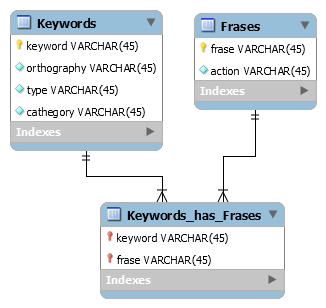
\includegraphics[width=0.5\textwidth]{modelo}
\end{wrapfigure}

Base de dados:
\begin{itemize}
\item Palavras-chave: tipo, categoria e ortografia de palavras-chave consideradas importante;\\
\item Frases: histórico de frases processadas.
\end{itemize}


\end{frame}


\subsection{Classificador de Respostas}
\begin{frame}{Classificador de Respostas}

\begin{itemize}
\item Após a análise do FreeLing, obtemos o PoS da frase de entrada. Depois, segue uma verificação ao modelo linguístico para ver se é detetado algum padrão. \vspace{2mm}

\item De seguida, passámos para a função que extrai as $features$ da frase. \vspace{2mm}

\item Estas features são uma combinação da verificação de padrões do modelo linguístico, bem como a comparação com outras frases já analisadas e também a presença de certas palavras-chave na frase.
\end{itemize}

\end{frame}

\end{document}


